% Study overview (vector, TikZ). Replaces the AI-drawn raster PNG of 2026-09-29.
% Carries no result numbers; every label is a Section III setup fact
% (sections/03_methodology.tex) or a Section IV measurement family name.
% Two rows: (1) data -> two architectures -> matched training; (2) evaluation families.
% Build:  bash paper/figures/overview/derle.sh   (latexmk + PNG preview + font check)
\documentclass[border=3pt]{standalone}
\usepackage[T1]{fontenc}
% helvet'in italik TFM'leri bu kurulumda eksik (phvro8t); Latin Modern sans kullanilir.
\IfFileExists{lmodern.sty}{\usepackage{lmodern}}{}
\renewcommand{\familydefault}{\sfdefault}
\usepackage{amsmath,amssymb}
\usepackage{tikz}
\usetikzlibrary{positioning,fit,arrows.meta,calc,backgrounds}

\definecolor{cnn}{RGB}{15,98,254}
\definecolor{vit}{RGB}{218,30,40}
\definecolor{ink}{RGB}{35,35,35}
\definecolor{mute}{RGB}{110,110,110}
\definecolor{pane}{RGB}{247,248,250}
\hyphenpenalty=10000 \exhyphenpenalty=10000

\begin{document}
\begin{tikzpicture}[
  font=\footnotesize, text=ink,
  >={Stealth[length=4.5pt,width=3.5pt]},
  every node/.style={align=center},
  blk/.style={draw=ink!65, fill=white, rounded corners=2pt, inner sep=3.5pt,
              text width=#1, minimum height=10mm},
  cont/.style={draw=#1, line width=0.9pt, rounded corners=4pt, inner sep=5pt, fill=pane},
  arr/.style={->, line width=0.8pt, draw=ink!70},
  ttl/.style={font=\small\bfseries, text=#1, inner sep=1pt, anchor=south west},
  sub/.style={font=\scriptsize, text=mute},
]

% ================================================================ ROW 1 =====
% ---------------------------------------------------------------- data ------
\node[blk=2.75cm, minimum height=46mm, fill=pane] (data) at (0,0) {%
  \rule{0pt}{15mm}% room for the thumbnails
  {\small\bfseries CIFAR-10}\\[2pt]
  \mbox{$32{\times}32{\times}3$, 10 classes}\\[4pt]
  50{,}000 training /\\
  10{,}000 test images\\[4pt]
  {\color{mute}2{,}000-image\\validation split\\held out before\\\emph{any} training stage}};
% real test images 0-3 (cifar_thumbs.py, nearest-neighbour upscaling)
\node[anchor=north, inner sep=0] (thumbs) at ($(data.north)+(0,-2.4mm)$) {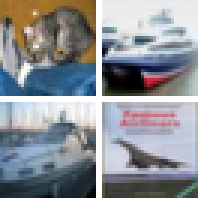
\includegraphics[width=11mm]{cifar_thumbs.png}};
\node[anchor=north, inner sep=0, font=\tiny, text=mute] at ($(thumbs.south)+(0,-0.6mm)$) {test images 0--3};

% ------------------------------------------------------------ CNN branch ----
\node[blk=1.70cm, draw=cnn] (c1) at (4.05, 2.35) {$3\times3$\\conv stem};
\node[blk=2.10cm, draw=cnn, right=3mm of c1] (c2) {8 residual blocks\\(4 stages)};
\node[blk=2.30cm, draw=cnn, right=3mm of c2] (c3) {global avg.\ pool + FC\\(10 classes)};
\begin{scope}[on background layer]
  \node[cont=cnn, fit=(c1)(c2)(c3), inner ysep=7pt, yshift=1.5pt] (cnnbox) {};
\end{scope}
\node[ttl=cnn] at ($(cnnbox.north west)+(1mm,0)$) {ResNet-18 \quad {\normalfont\footnotesize\color{mute}11.2M parameters}};
\draw[arr, draw=cnn] (c1) -- (c2);
\draw[arr, draw=cnn] (c2) -- (c3);

% ------------------------------------------------------------ ViT branch ----
\node[blk=1.55cm, draw=vit] (v1) at (3.80, -2.35) {bilinear\\upsampling\\$32\rightarrow224$};
\node[blk=1.95cm, draw=vit, right=3mm of v1] (v2) {$16\times16$ patches\\196 tokens + CLS\\dim 192};
\node[blk=1.95cm, draw=vit, right=3mm of v2] (v3) {12 Transformer\\blocks, 3 heads,\\MLP ratio 4};
\node[blk=1.35cm, draw=vit, right=3mm of v3] (v4) {CLS head\\(10 classes)};
\begin{scope}[on background layer]
  \node[cont=vit, fit=(v1)(v2)(v3)(v4), inner ysep=7pt, yshift=1.5pt] (vitbox) {};
\end{scope}
\node[ttl=vit] at ($(vitbox.north west)+(1mm,0)$) {ViT-Tiny \quad {\normalfont\footnotesize\color{mute}5.7M parameters, trained from scratch}};
\draw[arr, draw=vit] (v1) -- (v2);
\draw[arr, draw=vit] (v2) -- (v3);
\draw[arr, draw=vit] (v3) -- (v4);

% data -> branches
\draw[arr] (data.east) -- ++(4mm,0) |- (cnnbox.west);
\draw[arr] (data.east) -- ++(4mm,0) |- (vitbox.west);

% ------------------------------------------------------- training box ------
\node[blk=3.05cm, minimum height=62mm, fill=pane, draw=ink!65, line width=0.9pt, rounded corners=4pt]
  (train) at ($(vitbox.east)+(2.45cm,2.35)$) {%
  {\small\bfseries Matched training recipe}\\[5pt]
  {\color{mute}stage 1}\ \ clean training\\(200 epochs)\\[4pt]
  {\color{mute}stage 2}\ \ adversarial fine-tuning\\($\le$100 epochs, early stopping)\\
  inner attack PGD-10\\\mbox{$\varepsilon=8/255$, $\alpha=2/255$}\\
  loss $(1{-}\lambda)\,\mathrm{CE}(x)$\\$+\;\lambda\,\mathrm{CE}(x_{\mathrm{adv}})$, \ $\lambda=0.5$\\[4pt]
  3 independent runs\\per architecture\\[4pt]
  {\color{mute}checkpoint: best PGD-10\\accuracy on the held-out\\validation split}};
\begin{scope}[on background layer]
  \draw[ink!35, rounded corners=4pt] ($(train.south west)+(1.3mm,-1.3mm)$) rectangle ($(train.north east)+(1.3mm,-1.3mm)$);
  \draw[ink!20, rounded corners=4pt] ($(train.south west)+(2.6mm,-2.6mm)$) rectangle ($(train.north east)+(2.6mm,-2.6mm)$);
\end{scope}
\draw[arr, draw=cnn] (cnnbox.east) -- ++(3.5mm,0) |- ($(train.west)+(0,8mm)$);
\draw[arr, draw=vit] (vitbox.east) -- ++(3.5mm,0) |- ($(train.west)+(0,-8mm)$);

% ================================================================ ROW 2 =====
% five measurement families in a row, icon above each label box
\coordinate (rowy) at ($(vitbox.south west)+(0,-2.45cm)$);
\node[blk=2.85cm, minimum height=15.5mm, anchor=west] (e1) at (rowy -| data.west) {white-box robust accuracy\\PGD-10 and AutoAttack};
\node[blk=2.85cm, minimum height=15.5mm, right=3mm of e1] (e2) {conditional decomposition\\robust $=$ clean $\times$\\conditioned survival};
\node[blk=3.40cm, minimum height=15.5mm, right=3mm of e2] (e3) {transfer under four conditioning protocols\\raw $\supset$ target-correct $\supset$\\both-correct $\supset$ successful-source};
\node[blk=2.85cm, minimum height=15.5mm, right=3mm of e3] (e4) {gradient structure\\sparsity, alignment,\\spatial locality};
\node[blk=2.95cm, minimum height=15.5mm, right=3mm of e4] (e5) {depth profile\\block-wise feature drift,\\CLS attention entropy};
\begin{scope}[on background layer]
  \node[cont=ink!65, fit=(e1)(e5), inner xsep=5pt, inner ysep=7pt] (evalbox) {};
\end{scope}
\node[ttl=ink] at ($(evalbox.north west)+(1mm,0)$) {Evaluation \quad {\normalfont\footnotesize\color{mute}full test set, per-sample logging ($n=10{,}000$); the four protocols re-score the same records}};
\draw[arr] (train.south) -- (train.south |- evalbox.north);

% ------------------------------------------------------ bottom strip -------
\node[sub, text width=17.2cm, anchor=north, align=left, inner sep=2pt]
  at ($(evalbox.south)+(0,-2.5mm)$) {%
  \textbf{Replications and controls.}\;
  The whole design is repeated on CIFAR-100 (three runs per architecture) and SVHN (two runs); the CIFAR-10 checkpoints are re-evaluated under an $L_2$ budget ($\varepsilon=0.5$);
  a RobustBench WideResNet-28-10 checkpoint enters only as the third model of the $3\times3$ transfer matrix; the checkpoint-selection rule is varied on a fixed training trajectory.};

\end{tikzpicture}
\end{document}
